\documentclass[twoside]{book}

% Packages required by doxygen
\usepackage{calc}
\usepackage{doxygen}
\usepackage{graphicx}
\usepackage[utf8]{inputenc}
\usepackage{makeidx}
\usepackage{multicol}
\usepackage{multirow}
\usepackage{textcomp}
\usepackage[table]{xcolor}

% Font selection
\usepackage[T1]{fontenc}
\usepackage{mathptmx}
\usepackage[scaled=.90]{helvet}
\usepackage{courier}
\usepackage{amssymb}
\usepackage{sectsty}
\renewcommand{\familydefault}{\sfdefault}
\allsectionsfont{%
  \fontseries{bc}\selectfont%
  \color{darkgray}%
}
\renewcommand{\DoxyLabelFont}{%
  \fontseries{bc}\selectfont%
  \color{darkgray}%
}

% Page & text layout
\usepackage{geometry}
\geometry{%
  a4paper,%
  top=2.5cm,%
  bottom=2.5cm,%
  left=2.5cm,%
  right=2.5cm%
}
\tolerance=750
\hfuzz=15pt
\hbadness=750
\setlength{\emergencystretch}{15pt}
\setlength{\parindent}{0cm}
\setlength{\parskip}{0.2cm}
\makeatletter
\renewcommand{\paragraph}{%
  \@startsection{paragraph}{4}{0ex}{-1.0ex}{1.0ex}{%
    \normalfont\normalsize\bfseries\SS@parafont%
  }%
}
\renewcommand{\subparagraph}{%
  \@startsection{subparagraph}{5}{0ex}{-1.0ex}{1.0ex}{%
    \normalfont\normalsize\bfseries\SS@subparafont%
  }%
}
\makeatother

% Headers & footers
\usepackage{fancyhdr}
\pagestyle{fancyplain}
\fancyhead[LE]{\fancyplain{}{\bfseries\thepage}}
\fancyhead[CE]{\fancyplain{}{}}
\fancyhead[RE]{\fancyplain{}{\bfseries\leftmark}}
\fancyhead[LO]{\fancyplain{}{\bfseries\rightmark}}
\fancyhead[CO]{\fancyplain{}{}}
\fancyhead[RO]{\fancyplain{}{\bfseries\thepage}}
\fancyfoot[LE]{\fancyplain{}{}}
\fancyfoot[CE]{\fancyplain{}{}}
\fancyfoot[RE]{\fancyplain{}{\bfseries\scriptsize Generated on Fri Jul 1 2016 18\-:19\-:20 for R\-A\-P\-P Platform Tests -\/ Human Detection by Doxygen }}
\fancyfoot[LO]{\fancyplain{}{\bfseries\scriptsize Generated on Fri Jul 1 2016 18\-:19\-:20 for R\-A\-P\-P Platform Tests -\/ Human Detection by Doxygen }}
\fancyfoot[CO]{\fancyplain{}{}}
\fancyfoot[RO]{\fancyplain{}{}}
\renewcommand{\footrulewidth}{0.4pt}
\renewcommand{\chaptermark}[1]{%
  \markboth{#1}{}%
}
\renewcommand{\sectionmark}[1]{%
  \markright{\thesection\ #1}%
}

% Indices & bibliography
\usepackage{natbib}
\usepackage[titles]{tocloft}
\setcounter{tocdepth}{3}
\setcounter{secnumdepth}{5}
\makeindex

% Hyperlinks (required, but should be loaded last)
\usepackage{ifpdf}
\ifpdf
  \usepackage[pdftex,pagebackref=true]{hyperref}
\else
  \usepackage[ps2pdf,pagebackref=true]{hyperref}
\fi
\hypersetup{%
  colorlinks=true,%
  linkcolor=blue,%
  citecolor=blue,%
  unicode%
}

% Custom commands
\newcommand{\clearemptydoublepage}{%
  \newpage{\pagestyle{empty}\cleardoublepage}%
}


%===== C O N T E N T S =====

\begin{document}

% Titlepage & ToC
\hypersetup{pageanchor=false}
\pagenumbering{roman}
\begin{titlepage}
\vspace*{7cm}
\begin{center}%
{\Large R\-A\-P\-P Platform Tests -\/ Human Detection \\[1ex]\large v0.\-5.\-5 }\\
\vspace*{1cm}
{\large Generated by Doxygen 1.8.6}\\
\vspace*{0.5cm}
{\small Fri Jul 1 2016 18:19:20}\\
\end{center}
\end{titlepage}
\clearemptydoublepage
\tableofcontents
\clearemptydoublepage
\pagenumbering{arabic}
\hypersetup{pageanchor=true}

%--- Begin generated contents ---
\chapter{Namespace Index}
\section{Namespace List}
Here is a list of all namespaces with brief descriptions\-:\begin{DoxyCompactList}
\item\contentsline{section}{\hyperlink{namespacecognitive__exercise}{cognitive\-\_\-exercise} }{\pageref{namespacecognitive__exercise}}{}
\item\contentsline{section}{\hyperlink{namespacecognitive__exercise__main}{cognitive\-\_\-exercise\-\_\-main} }{\pageref{namespacecognitive__exercise__main}}{}
\item\contentsline{section}{\hyperlink{namespacemysql__wrapper}{mysql\-\_\-wrapper} }{\pageref{namespacemysql__wrapper}}{}
\item\contentsline{section}{\hyperlink{namespacemysql__wrapper__main}{mysql\-\_\-wrapper\-\_\-main} }{\pageref{namespacemysql__wrapper__main}}{}
\item\contentsline{section}{\hyperlink{namespacerapp__audio__processing}{rapp\-\_\-audio\-\_\-processing} }{\pageref{namespacerapp__audio__processing}}{}
\item\contentsline{section}{\hyperlink{namespacerapp__audio__processing_1_1rapp__audio__processing}{rapp\-\_\-audio\-\_\-processing.\-rapp\-\_\-audio\-\_\-processing} }{\pageref{namespacerapp__audio__processing_1_1rapp__audio__processing}}{}
\item\contentsline{section}{\hyperlink{namespacerapp__audio__processing_1_1rapp__detect__silence}{rapp\-\_\-audio\-\_\-processing.\-rapp\-\_\-detect\-\_\-silence} }{\pageref{namespacerapp__audio__processing_1_1rapp__detect__silence}}{}
\item\contentsline{section}{\hyperlink{namespacerapp__audio__processing_1_1rapp__energy__denoise}{rapp\-\_\-audio\-\_\-processing.\-rapp\-\_\-energy\-\_\-denoise} }{\pageref{namespacerapp__audio__processing_1_1rapp__energy__denoise}}{}
\item\contentsline{section}{\hyperlink{namespacerapp__audio__processing_1_1rapp__set__noise__profile}{rapp\-\_\-audio\-\_\-processing.\-rapp\-\_\-set\-\_\-noise\-\_\-profile} }{\pageref{namespacerapp__audio__processing_1_1rapp__set__noise__profile}}{}
\item\contentsline{section}{\hyperlink{namespacerapp__audio__processing_1_1rapp__sox__denoise}{rapp\-\_\-audio\-\_\-processing.\-rapp\-\_\-sox\-\_\-denoise} }{\pageref{namespacerapp__audio__processing_1_1rapp__sox__denoise}}{}
\item\contentsline{section}{\hyperlink{namespacerapp__audio__processing_1_1rapp__transform__audio}{rapp\-\_\-audio\-\_\-processing.\-rapp\-\_\-transform\-\_\-audio} }{\pageref{namespacerapp__audio__processing_1_1rapp__transform__audio}}{}
\item\contentsline{section}{\hyperlink{namespacerapp__audio__processing_1_1rapp__utilities}{rapp\-\_\-audio\-\_\-processing.\-rapp\-\_\-utilities} }{\pageref{namespacerapp__audio__processing_1_1rapp__utilities}}{}
\item\contentsline{section}{\hyperlink{namespacerapp__exceptions}{rapp\-\_\-exceptions} }{\pageref{namespacerapp__exceptions}}{}
\item\contentsline{section}{\hyperlink{namespacerapp__speech__detection__sphinx4}{rapp\-\_\-speech\-\_\-detection\-\_\-sphinx4} }{\pageref{namespacerapp__speech__detection__sphinx4}}{}
\item\contentsline{section}{\hyperlink{namespacerapp__speech__detection__sphinx4_1_1english__support}{rapp\-\_\-speech\-\_\-detection\-\_\-sphinx4.\-english\-\_\-support} }{\pageref{namespacerapp__speech__detection__sphinx4_1_1english__support}}{}
\item\contentsline{section}{\hyperlink{namespacerapp__speech__detection__sphinx4_1_1global__parameters}{rapp\-\_\-speech\-\_\-detection\-\_\-sphinx4.\-global\-\_\-parameters} }{\pageref{namespacerapp__speech__detection__sphinx4_1_1global__parameters}}{}
\item\contentsline{section}{\hyperlink{namespacerapp__speech__detection__sphinx4_1_1greek__support}{rapp\-\_\-speech\-\_\-detection\-\_\-sphinx4.\-greek\-\_\-support} }{\pageref{namespacerapp__speech__detection__sphinx4_1_1greek__support}}{}
\item\contentsline{section}{\hyperlink{namespacerapp__speech__detection__sphinx4_1_1limited__vocabulary__creator}{rapp\-\_\-speech\-\_\-detection\-\_\-sphinx4.\-limited\-\_\-vocabulary\-\_\-creator} }{\pageref{namespacerapp__speech__detection__sphinx4_1_1limited__vocabulary__creator}}{}
\item\contentsline{section}{\hyperlink{namespacerapp__speech__detection__sphinx4_1_1rapp__exceptions}{rapp\-\_\-speech\-\_\-detection\-\_\-sphinx4.\-rapp\-\_\-exceptions} }{\pageref{namespacerapp__speech__detection__sphinx4_1_1rapp__exceptions}}{}
\item\contentsline{section}{\hyperlink{namespacerapp__speech__detection__sphinx4_1_1rapp__tools}{rapp\-\_\-speech\-\_\-detection\-\_\-sphinx4.\-rapp\-\_\-tools} }{\pageref{namespacerapp__speech__detection__sphinx4_1_1rapp__tools}}{}
\item\contentsline{section}{\hyperlink{namespacerapp__speech__detection__sphinx4_1_1speech__recognition__sphinx4}{rapp\-\_\-speech\-\_\-detection\-\_\-sphinx4.\-speech\-\_\-recognition\-\_\-sphinx4} }{\pageref{namespacerapp__speech__detection__sphinx4_1_1speech__recognition__sphinx4}}{}
\item\contentsline{section}{\hyperlink{namespacerapp__speech__detection__sphinx4_1_1speech__recognition__sphinx4__handler__node}{rapp\-\_\-speech\-\_\-detection\-\_\-sphinx4.\-speech\-\_\-recognition\-\_\-sphinx4\-\_\-handler\-\_\-node} }{\pageref{namespacerapp__speech__detection__sphinx4_1_1speech__recognition__sphinx4__handler__node}}{}
\item\contentsline{section}{\hyperlink{namespacerapp__speech__detection__sphinx4_1_1sphinx4__configuration__params}{rapp\-\_\-speech\-\_\-detection\-\_\-sphinx4.\-sphinx4\-\_\-configuration\-\_\-params} }{\pageref{namespacerapp__speech__detection__sphinx4_1_1sphinx4__configuration__params}}{}
\item\contentsline{section}{\hyperlink{namespacerapp__speech__detection__sphinx4_1_1sphinx4__wrapper}{rapp\-\_\-speech\-\_\-detection\-\_\-sphinx4.\-sphinx4\-\_\-wrapper} }{\pageref{namespacerapp__speech__detection__sphinx4_1_1sphinx4__wrapper}}{}
\item\contentsline{section}{\hyperlink{namespacespeech__recognition__google}{speech\-\_\-recognition\-\_\-google} }{\pageref{namespacespeech__recognition__google}}{}
\item\contentsline{section}{\hyperlink{namespacetext__to__speech__espeak}{text\-\_\-to\-\_\-speech\-\_\-espeak} }{\pageref{namespacetext__to__speech__espeak}}{}
\end{DoxyCompactList}

\chapter{Hierarchical Index}
\section{Class Hierarchy}
This inheritance list is sorted roughly, but not completely, alphabetically\-:\begin{DoxyCompactList}
\item Test\begin{DoxyCompactList}
\item \contentsline{section}{Door\-Check\-Test}{\pageref{classDoorCheckTest}}{}
\item \contentsline{section}{Light\-Check\-Test}{\pageref{classLightCheckTest}}{}
\end{DoxyCompactList}
\item Test\-Case\begin{DoxyCompactList}
\item \contentsline{section}{functional\-\_\-tests.\-Hazard\-Detection\-Func}{\pageref{classfunctional__tests_1_1HazardDetectionFunc}}{}
\end{DoxyCompactList}
\end{DoxyCompactList}

\chapter{Class Index}
\section{Class List}
Here are the classes, structs, unions and interfaces with brief descriptions\-:\begin{DoxyCompactList}
\item\contentsline{section}{\hyperlink{classgoogle__news__explorer__test_1_1TestGoogleNewsExplorer}{google\-\_\-news\-\_\-explorer\-\_\-test.\-Test\-Google\-News\-Explorer} }{\pageref{classgoogle__news__explorer__test_1_1TestGoogleNewsExplorer}}{}
\end{DoxyCompactList}

\chapter{File Index}
\section{File List}
Here is a list of all files with brief descriptions\-:\begin{DoxyCompactList}
\item\contentsline{section}{/home/travis/rapp\-\_\-temp/rapp-\/api/cpp/examples/\hyperlink{face__detect_8cpp}{face\-\_\-detect.\-cpp} }{\pageref{face__detect_8cpp}}{}
\item\contentsline{section}{/home/travis/rapp\-\_\-temp/rapp-\/api/cpp/examples/\hyperlink{fetch__data_8cpp}{fetch\-\_\-data.\-cpp} }{\pageref{fetch__data_8cpp}}{}
\item\contentsline{section}{/home/travis/rapp\-\_\-temp/rapp-\/api/cpp/examples/\hyperlink{ontology__example_8cpp}{ontology\-\_\-example.\-cpp} }{\pageref{ontology__example_8cpp}}{}
\item\contentsline{section}{/home/travis/rapp\-\_\-temp/rapp-\/api/cpp/examples/\hyperlink{picture__example_8cpp}{picture\-\_\-example.\-cpp} }{\pageref{picture__example_8cpp}}{}
\item\contentsline{section}{/home/travis/rapp\-\_\-temp/rapp-\/api/cpp/examples/\hyperlink{qr__detect_8cpp}{qr\-\_\-detect.\-cpp} }{\pageref{qr__detect_8cpp}}{}
\item\contentsline{section}{/home/travis/rapp\-\_\-temp/rapp-\/api/cpp/examples/\hyperlink{set__denoise__example_8cpp}{set\-\_\-denoise\-\_\-example.\-cpp} }{\pageref{set__denoise__example_8cpp}}{}
\item\contentsline{section}{/home/travis/rapp\-\_\-temp/rapp-\/api/cpp/examples/\hyperlink{speech__to__text_8cpp}{speech\-\_\-to\-\_\-text.\-cpp} }{\pageref{speech__to__text_8cpp}}{}
\item\contentsline{section}{/home/travis/rapp\-\_\-temp/rapp-\/api/cpp/includes/cloud/face\-Detector/\hyperlink{faceDetector_8hpp}{face\-Detector.\-hpp} }{\pageref{faceDetector_8hpp}}{}
\item\contentsline{section}{/home/travis/rapp\-\_\-temp/rapp-\/api/cpp/includes/cloud/face\-Detector/\hyperlink{cloud_2faceDetector_2Includes_8ihh}{Includes.\-ihh} }{\pageref{cloud_2faceDetector_2Includes_8ihh}}{}
\item\contentsline{section}{/home/travis/rapp\-\_\-temp/rapp-\/api/cpp/includes/cloud/fetch\-Personal\-Data/\hyperlink{fetchPersonalData_8hpp}{fetch\-Personal\-Data.\-hpp} }{\pageref{fetchPersonalData_8hpp}}{}
\item\contentsline{section}{/home/travis/rapp\-\_\-temp/rapp-\/api/cpp/includes/cloud/fetch\-Personal\-Data/\hyperlink{cloud_2fetchPersonalData_2Includes_8ihh}{Includes.\-ihh} }{\pageref{cloud_2fetchPersonalData_2Includes_8ihh}}{}
\item\contentsline{section}{/home/travis/rapp\-\_\-temp/rapp-\/api/cpp/includes/cloud/ontology\-Is\-Sub\-Super\-Class\-Of/\hyperlink{cloud_2ontologyIsSubSuperClassOf_2Includes_8ihh}{Includes.\-ihh} }{\pageref{cloud_2ontologyIsSubSuperClassOf_2Includes_8ihh}}{}
\item\contentsline{section}{/home/travis/rapp\-\_\-temp/rapp-\/api/cpp/includes/cloud/ontology\-Is\-Sub\-Super\-Class\-Of/\hyperlink{ontologyIsSubSuperClassOf_8hpp}{ontology\-Is\-Sub\-Super\-Class\-Of.\-hpp} }{\pageref{ontologyIsSubSuperClassOf_8hpp}}{}
\item\contentsline{section}{/home/travis/rapp\-\_\-temp/rapp-\/api/cpp/includes/cloud/ontology\-Sub\-Classes\-Of/\hyperlink{cloud_2ontologySubClassesOf_2Includes_8ihh}{Includes.\-ihh} }{\pageref{cloud_2ontologySubClassesOf_2Includes_8ihh}}{}
\item\contentsline{section}{/home/travis/rapp\-\_\-temp/rapp-\/api/cpp/includes/cloud/ontology\-Sub\-Classes\-Of/\hyperlink{ontologySubClassesOf_8hpp}{ontology\-Sub\-Classes\-Of.\-hpp} }{\pageref{ontologySubClassesOf_8hpp}}{}
\item\contentsline{section}{/home/travis/rapp\-\_\-temp/rapp-\/api/cpp/includes/cloud/ontology\-Super\-Classes\-Of/\hyperlink{cloud_2ontologySuperClassesOf_2Includes_8ihh}{Includes.\-ihh} }{\pageref{cloud_2ontologySuperClassesOf_2Includes_8ihh}}{}
\item\contentsline{section}{/home/travis/rapp\-\_\-temp/rapp-\/api/cpp/includes/cloud/ontology\-Super\-Classes\-Of/\hyperlink{ontologySuperClassesOf_8hpp}{ontology\-Super\-Classes\-Of.\-hpp} }{\pageref{ontologySuperClassesOf_8hpp}}{}
\item\contentsline{section}{/home/travis/rapp\-\_\-temp/rapp-\/api/cpp/includes/cloud/qr\-Detector/\hyperlink{cloud_2qrDetector_2Includes_8ihh}{Includes.\-ihh} }{\pageref{cloud_2qrDetector_2Includes_8ihh}}{}
\item\contentsline{section}{/home/travis/rapp\-\_\-temp/rapp-\/api/cpp/includes/cloud/qr\-Detector/\hyperlink{qrDetector_8hpp}{qr\-Detector.\-hpp} }{\pageref{qrDetector_8hpp}}{}
\item\contentsline{section}{/home/travis/rapp\-\_\-temp/rapp-\/api/cpp/includes/cloud/set\-Denoise\-Profile/\hyperlink{cloud_2setDenoiseProfile_2Includes_8ihh}{Includes.\-ihh} }{\pageref{cloud_2setDenoiseProfile_2Includes_8ihh}}{}
\item\contentsline{section}{/home/travis/rapp\-\_\-temp/rapp-\/api/cpp/includes/cloud/set\-Denoise\-Profile/\hyperlink{setDenoiseProfile_8hpp}{set\-Denoise\-Profile.\-hpp} }{\pageref{setDenoiseProfile_8hpp}}{}
\item\contentsline{section}{/home/travis/rapp\-\_\-temp/rapp-\/api/cpp/includes/cloud/speech\-To\-Text/\hyperlink{cloud_2speechToText_2Includes_8ihh}{Includes.\-ihh} }{\pageref{cloud_2speechToText_2Includes_8ihh}}{}
\item\contentsline{section}{/home/travis/rapp\-\_\-temp/rapp-\/api/cpp/includes/cloud/speech\-To\-Text/\hyperlink{speechToText_8hpp}{speech\-To\-Text.\-hpp} }{\pageref{speechToText_8hpp}}{}
\item\contentsline{section}{/home/travis/rapp\-\_\-temp/rapp-\/api/cpp/includes/cloud/up\-Services/\hyperlink{cloud_2upServices_2Includes_8ihh}{Includes.\-ihh} }{\pageref{cloud_2upServices_2Includes_8ihh}}{}
\item\contentsline{section}{/home/travis/rapp\-\_\-temp/rapp-\/api/cpp/includes/cloud/up\-Services/\hyperlink{upServices_8hpp}{up\-Services.\-hpp} }{\pageref{upServices_8hpp}}{}
\item\contentsline{section}{/home/travis/rapp\-\_\-temp/rapp-\/api/cpp/includes/objects/audio/\hyperlink{audio_8hpp}{audio.\-hpp} }{\pageref{audio_8hpp}}{}
\item\contentsline{section}{/home/travis/rapp\-\_\-temp/rapp-\/api/cpp/includes/objects/audio/\hyperlink{objects_2audio_2Includes_8ihh}{Includes.\-ihh} }{\pageref{objects_2audio_2Includes_8ihh}}{}
\item\contentsline{section}{/home/travis/rapp\-\_\-temp/rapp-\/api/cpp/includes/objects/face/\hyperlink{face_8hpp}{face.\-hpp} }{\pageref{face_8hpp}}{}
\item\contentsline{section}{/home/travis/rapp\-\_\-temp/rapp-\/api/cpp/includes/objects/face/\hyperlink{objects_2face_2Includes_8ihh}{Includes.\-ihh} }{\pageref{objects_2face_2Includes_8ihh}}{}
\item\contentsline{section}{/home/travis/rapp\-\_\-temp/rapp-\/api/cpp/includes/objects/picture/\hyperlink{objects_2picture_2Includes_8ihh}{Includes.\-ihh} }{\pageref{objects_2picture_2Includes_8ihh}}{}
\item\contentsline{section}{/home/travis/rapp\-\_\-temp/rapp-\/api/cpp/includes/objects/picture/\hyperlink{picture_8hpp}{picture.\-hpp} }{\pageref{picture_8hpp}}{}
\item\contentsline{section}{/home/travis/rapp\-\_\-temp/rapp-\/api/cpp/includes/objects/qr\-Code/\hyperlink{objects_2qrCode_2Includes_8ihh}{Includes.\-ihh} }{\pageref{objects_2qrCode_2Includes_8ihh}}{}
\item\contentsline{section}{/home/travis/rapp\-\_\-temp/rapp-\/api/cpp/includes/objects/qr\-Code/\hyperlink{qrCode_8hpp}{qr\-Code.\-hpp} }{\pageref{qrCode_8hpp}}{}
\item\contentsline{section}{/home/travis/rapp\-\_\-temp/rapp-\/api/cpp/includes/robot/communication/\hyperlink{communication_8hpp}{communication.\-hpp} }{\pageref{communication_8hpp}}{}
\item\contentsline{section}{/home/travis/rapp\-\_\-temp/rapp-\/api/cpp/includes/robot/communication/\hyperlink{robot_2communication_2Includes_8ihh}{Includes.\-ihh} }{\pageref{robot_2communication_2Includes_8ihh}}{}
\item\contentsline{section}{/home/travis/rapp\-\_\-temp/rapp-\/api/cpp/includes/robot/nao/\hyperlink{robot_2nao_2Includes_8ihh}{Includes.\-ihh} }{\pageref{robot_2nao_2Includes_8ihh}}{}
\item\contentsline{section}{/home/travis/rapp\-\_\-temp/rapp-\/api/cpp/includes/robot/nao/\hyperlink{nao_8hpp}{nao.\-hpp} }{\pageref{nao_8hpp}}{}
\item\contentsline{section}{/home/travis/rapp\-\_\-temp/rapp-\/api/cpp/includes/robot/navigation/\hyperlink{robot_2navigation_2Includes_8ihh}{Includes.\-ihh} }{\pageref{robot_2navigation_2Includes_8ihh}}{}
\item\contentsline{section}{/home/travis/rapp\-\_\-temp/rapp-\/api/cpp/includes/robot/navigation/\hyperlink{navigation_8hpp}{navigation.\-hpp} }{\pageref{navigation_8hpp}}{}
\item\contentsline{section}{/home/travis/rapp\-\_\-temp/rapp-\/api/cpp/includes/robot/proto/\hyperlink{robot_2proto_2Includes_8ihh}{Includes.\-ihh} }{\pageref{robot_2proto_2Includes_8ihh}}{}
\item\contentsline{section}{/home/travis/rapp\-\_\-temp/rapp-\/api/cpp/includes/robot/proto/\hyperlink{proto_8hpp}{proto.\-hpp} }{\pageref{proto_8hpp}}{}
\item\contentsline{section}{/home/travis/rapp\-\_\-temp/rapp-\/api/cpp/includes/robot/vision/\hyperlink{robot_2vision_2Includes_8ihh}{Includes.\-ihh} }{\pageref{robot_2vision_2Includes_8ihh}}{}
\item\contentsline{section}{/home/travis/rapp\-\_\-temp/rapp-\/api/cpp/includes/robot/vision/\hyperlink{vision_8hpp}{vision.\-hpp} }{\pageref{vision_8hpp}}{}
\item\contentsline{section}{/home/travis/rapp\-\_\-temp/rapp-\/api/cpp/includes/service/asio\-\_\-service\-\_\-http/\hyperlink{asio__service__http_8hpp}{asio\-\_\-service\-\_\-http.\-hpp} }{\pageref{asio__service__http_8hpp}}{}
\item\contentsline{section}{/home/travis/rapp\-\_\-temp/rapp-\/api/cpp/includes/service/asio\-\_\-service\-\_\-http/\hyperlink{service_2asio__service__http_2Includes_8ihh}{Includes.\-ihh} }{\pageref{service_2asio__service__http_2Includes_8ihh}}{}
\item\contentsline{section}{/home/travis/rapp\-\_\-temp/rapp-\/api/cpp/includes/service/asio\-\_\-service\-\_\-raw/\hyperlink{asio__service__raw_8cpp}{asio\-\_\-service\-\_\-raw.\-cpp} }{\pageref{asio__service__raw_8cpp}}{}
\item\contentsline{section}{/home/travis/rapp\-\_\-temp/rapp-\/api/cpp/includes/service/asio\-\_\-service\-\_\-raw/\hyperlink{asio__service__raw_8hpp}{asio\-\_\-service\-\_\-raw.\-hpp} }{\pageref{asio__service__raw_8hpp}}{}
\item\contentsline{section}{/home/travis/rapp\-\_\-temp/rapp-\/api/cpp/includes/service/asio\-\_\-service\-\_\-raw/\hyperlink{service_2asio__service__raw_2Includes_8ihh}{Includes.\-ihh} }{\pageref{service_2asio__service__raw_2Includes_8ihh}}{}
\item\contentsline{section}{/home/travis/rapp\-\_\-temp/rapp-\/api/cpp/includes/service/asio\-\_\-socket/\hyperlink{asio__socket_8hpp}{asio\-\_\-socket.\-hpp} }{\pageref{asio__socket_8hpp}}{}
\item\contentsline{section}{/home/travis/rapp\-\_\-temp/rapp-\/api/cpp/includes/service/asio\-\_\-socket/\hyperlink{service_2asio__socket_2Includes_8ihh}{Includes.\-ihh} }{\pageref{service_2asio__socket_2Includes_8ihh}}{}
\item\contentsline{section}{/home/travis/rapp\-\_\-temp/rapp-\/api/cpp/includes/service/globals/\hyperlink{globals_8hpp}{globals.\-hpp} }{\pageref{globals_8hpp}}{}
\item\contentsline{section}{/home/travis/rapp\-\_\-temp/rapp-\/api/cpp/includes/service/service\-\_\-controller/\hyperlink{service_2service__controller_2Includes_8ihh}{Includes.\-ihh} }{\pageref{service_2service__controller_2Includes_8ihh}}{}
\item\contentsline{section}{/home/travis/rapp\-\_\-temp/rapp-\/api/cpp/includes/service/service\-\_\-controller/\hyperlink{service__controller_8hpp}{service\-\_\-controller.\-hpp} }{\pageref{service__controller_8hpp}}{}
\item\contentsline{section}{/home/travis/rapp\-\_\-temp/rapp-\/api/python/\-Rapp\-Cloud/\hyperlink{____init_____8py}{\-\_\-\-\_\-init\-\_\-\-\_\-.\-py} }{\pageref{____init_____8py}}{}
\item\contentsline{section}{/home/travis/rapp\-\_\-temp/rapp-\/api/python/\-Rapp\-Cloud/\hyperlink{RappCloud_8py}{Rapp\-Cloud.\-py} }{\pageref{RappCloud_8py}}{}
\item\contentsline{section}{/home/travis/rapp\-\_\-temp/rapp-\/api/python/\-Rapp\-Cloud/\-Cloud\-Interface/\hyperlink{CloudInterface_2____init_____8py}{\-\_\-\-\_\-init\-\_\-\-\_\-.\-py} }{\pageref{CloudInterface_2____init_____8py}}{}
\item\contentsline{section}{/home/travis/rapp\-\_\-temp/rapp-\/api/python/\-Rapp\-Cloud/\-Cloud\-Interface/\hyperlink{CloudInterface_8py}{Cloud\-Interface.\-py} }{\pageref{CloudInterface_8py}}{}
\item\contentsline{section}{/home/travis/rapp\-\_\-temp/rapp-\/api/python/\-Rapp\-Cloud/\-Rand\-Str\-Gen/\hyperlink{RandStrGen_2____init_____8py}{\-\_\-\-\_\-init\-\_\-\-\_\-.\-py} }{\pageref{RandStrGen_2____init_____8py}}{}
\item\contentsline{section}{/home/travis/rapp\-\_\-temp/rapp-\/api/python/\-Rapp\-Cloud/\-Rand\-Str\-Gen/\hyperlink{RandStrGen_8py}{Rand\-Str\-Gen.\-py} }{\pageref{RandStrGen_8py}}{}
\end{DoxyCompactList}

\chapter{Namespace Documentation}
\hypertarget{namespacefunctional__tests}{\section{functional\-\_\-tests Namespace Reference}
\label{namespacefunctional__tests}\index{functional\-\_\-tests@{functional\-\_\-tests}}
}
\subsection*{Classes}
\begin{DoxyCompactItemize}
\item 
class \hyperlink{classfunctional__tests_1_1SpeechToTextFunc}{Speech\-To\-Text\-Func}
\begin{DoxyCompactList}\small\item\em Inherits the unittest.\-Test\-Case class in order to offer functional tests functionality. \end{DoxyCompactList}\end{DoxyCompactItemize}
\subsection*{Variables}
\begin{DoxyCompactItemize}
\item 
string \hyperlink{namespacefunctional__tests_a78507f367d6307db1c1633379cbccc35}{P\-K\-G} = 'rapp\-\_\-speech\-\_\-detection\-\_\-google'
\end{DoxyCompactItemize}


\subsection{Variable Documentation}
\hypertarget{namespacefunctional__tests_a78507f367d6307db1c1633379cbccc35}{\index{functional\-\_\-tests@{functional\-\_\-tests}!P\-K\-G@{P\-K\-G}}
\index{P\-K\-G@{P\-K\-G}!functional_tests@{functional\-\_\-tests}}
\subsubsection[{P\-K\-G}]{\setlength{\rightskip}{0pt plus 5cm}string functional\-\_\-tests.\-P\-K\-G = 'rapp\-\_\-speech\-\_\-detection\-\_\-google'}}\label{namespacefunctional__tests_a78507f367d6307db1c1633379cbccc35}


Definition at line 18 of file functional\-\_\-tests.\-py.


\chapter{Class Documentation}
\hypertarget{classHumanDetectionTest}{\section{Human\-Detection\-Test Class Reference}
\label{classHumanDetectionTest}\index{Human\-Detection\-Test@{Human\-Detection\-Test}}
}


Handles the human detection unit testing using gtests.  




Inheritance diagram for Human\-Detection\-Test\-:
\nopagebreak
\begin{figure}[H]
\begin{center}
\leavevmode
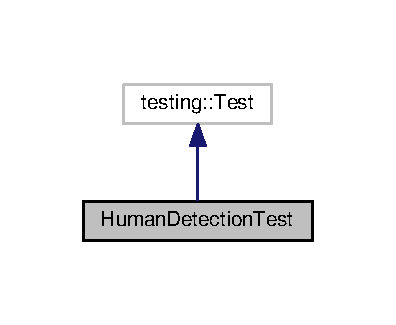
\includegraphics[width=190pt]{classHumanDetectionTest__inherit__graph}
\end{center}
\end{figure}


Collaboration diagram for Human\-Detection\-Test\-:
\nopagebreak
\begin{figure}[H]
\begin{center}
\leavevmode
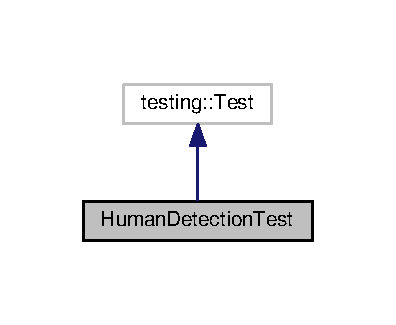
\includegraphics[width=190pt]{classHumanDetectionTest__coll__graph}
\end{center}
\end{figure}
\subsection*{Protected Member Functions}
\begin{DoxyCompactItemize}
\item 
\hyperlink{classHumanDetectionTest_a3c57e54c0bd3bdcd1d3835463d1cb3a7}{Human\-Detection\-Test} ()
\begin{DoxyCompactList}\small\item\em Default constructor. \end{DoxyCompactList}\item 
virtual void \hyperlink{classHumanDetectionTest_a2f61d8cd6c5e18e3f52440f95f3746f7}{Set\-Up} ()
\begin{DoxyCompactList}\small\item\em Sets up the class variables for each unit test call. \end{DoxyCompactList}\item 
virtual void \hyperlink{classHumanDetectionTest_a6cd19bdb532d8cea1292b67ea862db88}{Tear\-Down} ()
\begin{DoxyCompactList}\small\item\em This function is called after the termination of each test. Destroys the dynamically alloced variables. \end{DoxyCompactList}\end{DoxyCompactItemize}
\subsection*{Protected Attributes}
\begin{DoxyCompactItemize}
\item 
Human\-Detector $\ast$ \hyperlink{classHumanDetectionTest_a052710732ae09a580f044ad2a0f1e9fc}{human\-\_\-detector\-\_\-}
\end{DoxyCompactItemize}


\subsection{Detailed Description}
Handles the human detection unit testing using gtests. 

Definition at line 27 of file unit\-\_\-tests.\-cpp.



\subsection{Constructor \& Destructor Documentation}
\hypertarget{classHumanDetectionTest_a3c57e54c0bd3bdcd1d3835463d1cb3a7}{\index{Human\-Detection\-Test@{Human\-Detection\-Test}!Human\-Detection\-Test@{Human\-Detection\-Test}}
\index{Human\-Detection\-Test@{Human\-Detection\-Test}!HumanDetectionTest@{Human\-Detection\-Test}}
\subsubsection[{Human\-Detection\-Test}]{\setlength{\rightskip}{0pt plus 5cm}Human\-Detection\-Test\-::\-Human\-Detection\-Test (
\begin{DoxyParamCaption}
{}
\end{DoxyParamCaption}
)\hspace{0.3cm}{\ttfamily [inline]}, {\ttfamily [protected]}}}\label{classHumanDetectionTest_a3c57e54c0bd3bdcd1d3835463d1cb3a7}


Default constructor. 



Definition at line 34 of file unit\-\_\-tests.\-cpp.



\subsection{Member Function Documentation}
\hypertarget{classHumanDetectionTest_a2f61d8cd6c5e18e3f52440f95f3746f7}{\index{Human\-Detection\-Test@{Human\-Detection\-Test}!Set\-Up@{Set\-Up}}
\index{Set\-Up@{Set\-Up}!HumanDetectionTest@{Human\-Detection\-Test}}
\subsubsection[{Set\-Up}]{\setlength{\rightskip}{0pt plus 5cm}virtual void Human\-Detection\-Test\-::\-Set\-Up (
\begin{DoxyParamCaption}
{}
\end{DoxyParamCaption}
)\hspace{0.3cm}{\ttfamily [inline]}, {\ttfamily [protected]}, {\ttfamily [virtual]}}}\label{classHumanDetectionTest_a2f61d8cd6c5e18e3f52440f95f3746f7}


Sets up the class variables for each unit test call. 



Definition at line 40 of file unit\-\_\-tests.\-cpp.

\hypertarget{classHumanDetectionTest_a6cd19bdb532d8cea1292b67ea862db88}{\index{Human\-Detection\-Test@{Human\-Detection\-Test}!Tear\-Down@{Tear\-Down}}
\index{Tear\-Down@{Tear\-Down}!HumanDetectionTest@{Human\-Detection\-Test}}
\subsubsection[{Tear\-Down}]{\setlength{\rightskip}{0pt plus 5cm}virtual void Human\-Detection\-Test\-::\-Tear\-Down (
\begin{DoxyParamCaption}
{}
\end{DoxyParamCaption}
)\hspace{0.3cm}{\ttfamily [inline]}, {\ttfamily [protected]}, {\ttfamily [virtual]}}}\label{classHumanDetectionTest_a6cd19bdb532d8cea1292b67ea862db88}


This function is called after the termination of each test. Destroys the dynamically alloced variables. 



Definition at line 48 of file unit\-\_\-tests.\-cpp.



\subsection{Member Data Documentation}
\hypertarget{classHumanDetectionTest_a052710732ae09a580f044ad2a0f1e9fc}{\index{Human\-Detection\-Test@{Human\-Detection\-Test}!human\-\_\-detector\-\_\-@{human\-\_\-detector\-\_\-}}
\index{human\-\_\-detector\-\_\-@{human\-\_\-detector\-\_\-}!HumanDetectionTest@{Human\-Detection\-Test}}
\subsubsection[{human\-\_\-detector\-\_\-}]{\setlength{\rightskip}{0pt plus 5cm}Human\-Detector$\ast$ Human\-Detection\-Test\-::human\-\_\-detector\-\_\-\hspace{0.3cm}{\ttfamily [protected]}}}\label{classHumanDetectionTest_a052710732ae09a580f044ad2a0f1e9fc}
Pointer of type Human\-Detector. Used to check its functions 

Definition at line 53 of file unit\-\_\-tests.\-cpp.



The documentation for this class was generated from the following file\-:\begin{DoxyCompactItemize}
\item 
/home/travis/rapp\-\_\-temp/rapp-\/platform/rapp\-\_\-human\-\_\-detection/tests/human\-\_\-detection/\hyperlink{unit__tests_8cpp}{unit\-\_\-tests.\-cpp}\end{DoxyCompactItemize}

\hypertarget{classfunctional__tests_1_1HumanDetFunc}{\section{functional\-\_\-tests.\-Human\-Det\-Func Class Reference}
\label{classfunctional__tests_1_1HumanDetFunc}\index{functional\-\_\-tests.\-Human\-Det\-Func@{functional\-\_\-tests.\-Human\-Det\-Func}}
}


Inheritance diagram for functional\-\_\-tests.\-Human\-Det\-Func\-:
\nopagebreak
\begin{figure}[H]
\begin{center}
\leavevmode
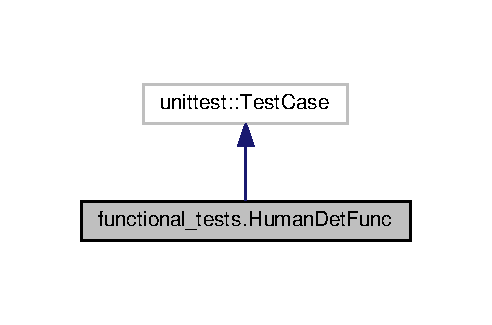
\includegraphics[width=236pt]{classfunctional__tests_1_1HumanDetFunc__inherit__graph}
\end{center}
\end{figure}


Collaboration diagram for functional\-\_\-tests.\-Human\-Det\-Func\-:
\nopagebreak
\begin{figure}[H]
\begin{center}
\leavevmode
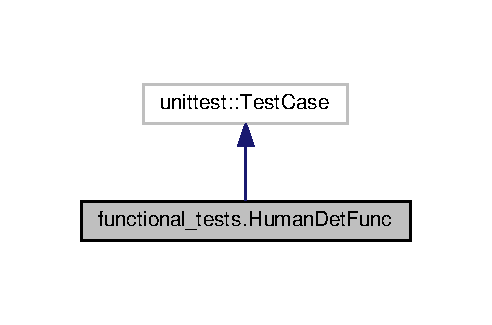
\includegraphics[width=236pt]{classfunctional__tests_1_1HumanDetFunc__coll__graph}
\end{center}
\end{figure}
\subsection*{Public Member Functions}
\begin{DoxyCompactItemize}
\item 
def \hyperlink{classfunctional__tests_1_1HumanDetFunc_aaa6e3a1a731f9585fab34d035c05b874}{test\-\_\-file\-Does\-Not\-Exist}
\begin{DoxyCompactList}\small\item\em Tests human detection with a non existent image. \end{DoxyCompactList}\item 
def \hyperlink{classfunctional__tests_1_1HumanDetFunc_a4fc900b3b0fdb6e604f9b8bdaae5296d}{test\-\_\-file\-Exists\-But\-It\-Audio}
\begin{DoxyCompactList}\small\item\em Tests human detection with an audio file. \end{DoxyCompactList}\item 
def \hyperlink{classfunctional__tests_1_1HumanDetFunc_a8074f58695d994f010ad333fed75068b}{test\-\_\-human\-Does\-Not\-Exist}
\begin{DoxyCompactList}\small\item\em Tests human detection with an image that does not contain humans. \end{DoxyCompactList}\item 
def \hyperlink{classfunctional__tests_1_1HumanDetFunc_a2736713be5cc1ddd091331d3306dfd0e}{test\-\_\-human\-Exists\-\_\-realistic}
\begin{DoxyCompactList}\small\item\em Tests human detection with a N\-A\-O captured image. \end{DoxyCompactList}\item 
def \hyperlink{classfunctional__tests_1_1HumanDetFunc_a6d8971bce2f04f8ea05f6d30e22b6d2c}{test\-\_\-human\-Exists\-\_\-stress}
\begin{DoxyCompactList}\small\item\em Tests human detection with a N\-A\-O captured image from almost 2 meters. \end{DoxyCompactList}\end{DoxyCompactItemize}


\subsection{Detailed Description}
\begin{DoxyVerb}Handles the human detection functional tests
\end{DoxyVerb}
 

Definition at line 32 of file functional\-\_\-tests.\-py.



\subsection{Member Function Documentation}
\hypertarget{classfunctional__tests_1_1HumanDetFunc_aaa6e3a1a731f9585fab34d035c05b874}{\index{functional\-\_\-tests\-::\-Human\-Det\-Func@{functional\-\_\-tests\-::\-Human\-Det\-Func}!test\-\_\-file\-Does\-Not\-Exist@{test\-\_\-file\-Does\-Not\-Exist}}
\index{test\-\_\-file\-Does\-Not\-Exist@{test\-\_\-file\-Does\-Not\-Exist}!functional_tests::HumanDetFunc@{functional\-\_\-tests\-::\-Human\-Det\-Func}}
\subsubsection[{test\-\_\-file\-Does\-Not\-Exist}]{\setlength{\rightskip}{0pt plus 5cm}def functional\-\_\-tests.\-Human\-Det\-Func.\-test\-\_\-file\-Does\-Not\-Exist (
\begin{DoxyParamCaption}
\item[{}]{self}
\end{DoxyParamCaption}
)}}\label{classfunctional__tests_1_1HumanDetFunc_aaa6e3a1a731f9585fab34d035c05b874}


Tests human detection with a non existent image. 

Should return 0 humans 

Definition at line 91 of file functional\-\_\-tests.\-py.

\hypertarget{classfunctional__tests_1_1HumanDetFunc_a4fc900b3b0fdb6e604f9b8bdaae5296d}{\index{functional\-\_\-tests\-::\-Human\-Det\-Func@{functional\-\_\-tests\-::\-Human\-Det\-Func}!test\-\_\-file\-Exists\-But\-It\-Audio@{test\-\_\-file\-Exists\-But\-It\-Audio}}
\index{test\-\_\-file\-Exists\-But\-It\-Audio@{test\-\_\-file\-Exists\-But\-It\-Audio}!functional_tests::HumanDetFunc@{functional\-\_\-tests\-::\-Human\-Det\-Func}}
\subsubsection[{test\-\_\-file\-Exists\-But\-It\-Audio}]{\setlength{\rightskip}{0pt plus 5cm}def functional\-\_\-tests.\-Human\-Det\-Func.\-test\-\_\-file\-Exists\-But\-It\-Audio (
\begin{DoxyParamCaption}
\item[{}]{self}
\end{DoxyParamCaption}
)}}\label{classfunctional__tests_1_1HumanDetFunc_a4fc900b3b0fdb6e604f9b8bdaae5296d}


Tests human detection with an audio file. 

Should not crush an return 0 humans 

Definition at line 104 of file functional\-\_\-tests.\-py.

\hypertarget{classfunctional__tests_1_1HumanDetFunc_a8074f58695d994f010ad333fed75068b}{\index{functional\-\_\-tests\-::\-Human\-Det\-Func@{functional\-\_\-tests\-::\-Human\-Det\-Func}!test\-\_\-human\-Does\-Not\-Exist@{test\-\_\-human\-Does\-Not\-Exist}}
\index{test\-\_\-human\-Does\-Not\-Exist@{test\-\_\-human\-Does\-Not\-Exist}!functional_tests::HumanDetFunc@{functional\-\_\-tests\-::\-Human\-Det\-Func}}
\subsubsection[{test\-\_\-human\-Does\-Not\-Exist}]{\setlength{\rightskip}{0pt plus 5cm}def functional\-\_\-tests.\-Human\-Det\-Func.\-test\-\_\-human\-Does\-Not\-Exist (
\begin{DoxyParamCaption}
\item[{}]{self}
\end{DoxyParamCaption}
)}}\label{classfunctional__tests_1_1HumanDetFunc_a8074f58695d994f010ad333fed75068b}


Tests human detection with an image that does not contain humans. 

Should return 0 humans 

Definition at line 78 of file functional\-\_\-tests.\-py.

\hypertarget{classfunctional__tests_1_1HumanDetFunc_a2736713be5cc1ddd091331d3306dfd0e}{\index{functional\-\_\-tests\-::\-Human\-Det\-Func@{functional\-\_\-tests\-::\-Human\-Det\-Func}!test\-\_\-human\-Exists\-\_\-realistic@{test\-\_\-human\-Exists\-\_\-realistic}}
\index{test\-\_\-human\-Exists\-\_\-realistic@{test\-\_\-human\-Exists\-\_\-realistic}!functional_tests::HumanDetFunc@{functional\-\_\-tests\-::\-Human\-Det\-Func}}
\subsubsection[{test\-\_\-human\-Exists\-\_\-realistic}]{\setlength{\rightskip}{0pt plus 5cm}def functional\-\_\-tests.\-Human\-Det\-Func.\-test\-\_\-human\-Exists\-\_\-realistic (
\begin{DoxyParamCaption}
\item[{}]{self}
\end{DoxyParamCaption}
)}}\label{classfunctional__tests_1_1HumanDetFunc_a2736713be5cc1ddd091331d3306dfd0e}


Tests human detection with a N\-A\-O captured image. 

Should return 1 human 

Definition at line 37 of file functional\-\_\-tests.\-py.

\hypertarget{classfunctional__tests_1_1HumanDetFunc_a6d8971bce2f04f8ea05f6d30e22b6d2c}{\index{functional\-\_\-tests\-::\-Human\-Det\-Func@{functional\-\_\-tests\-::\-Human\-Det\-Func}!test\-\_\-human\-Exists\-\_\-stress@{test\-\_\-human\-Exists\-\_\-stress}}
\index{test\-\_\-human\-Exists\-\_\-stress@{test\-\_\-human\-Exists\-\_\-stress}!functional_tests::HumanDetFunc@{functional\-\_\-tests\-::\-Human\-Det\-Func}}
\subsubsection[{test\-\_\-human\-Exists\-\_\-stress}]{\setlength{\rightskip}{0pt plus 5cm}def functional\-\_\-tests.\-Human\-Det\-Func.\-test\-\_\-human\-Exists\-\_\-stress (
\begin{DoxyParamCaption}
\item[{}]{self}
\end{DoxyParamCaption}
)}}\label{classfunctional__tests_1_1HumanDetFunc_a6d8971bce2f04f8ea05f6d30e22b6d2c}


Tests human detection with a N\-A\-O captured image from almost 2 meters. 

Should return 1 human D\-I\-S\-A\-B\-L\-E\-D -\/ Returned 2 def test\-\_\-human\-Exists\-\_\-realistic\-\_\-2(self)\-: rospack = rospkg.\-Ros\-Pack() human\-\_\-service = rospy.\-get\-\_\-param(\char`\"{}rapp\-\_\-human\-\_\-detection\-\_\-detect\-\_\-humans\-\_\-topic\char`\"{}) rospy.\-wait\-\_\-for\-\_\-service(human\-\_\-service) fd\-\_\-service = rospy.\-Service\-Proxy(human\-\_\-service, Human\-Detection\-Ros\-Srv) req = Human\-Detection\-Ros\-Srv\-Request() req.\-image\-Filename = rospack.\-get\-\_\-path('rapp\-\_\-testing\-\_\-tools') + \textbackslash{} '/test\-\_\-data/human\-\_\-detection\-\_\-samples/\-N\-A\-O\-\_\-picture\-\_\-10.png' response = fd\-\_\-service(req) humans\-\_\-num = len(response.\-humans\-\_\-up\-\_\-left) self.\-assert\-Equal( humans\-\_\-num, 1 ) Stress test for human detection. 20 calls in a row 

Definition at line 64 of file functional\-\_\-tests.\-py.



The documentation for this class was generated from the following file\-:\begin{DoxyCompactItemize}
\item 
/home/travis/rapp\-\_\-temp/rapp-\/platform/rapp\-\_\-human\-\_\-detection/tests/human\-\_\-detection/\hyperlink{functional__tests_8py}{functional\-\_\-tests.\-py}\end{DoxyCompactItemize}

\chapter{File Documentation}
\hypertarget{functional__tests_8py}{\section{/home/travis/rapp\-\_\-temp/rapp-\/platform/rapp\-\_\-speech\-\_\-detection\-\_\-google/tests/speech\-\_\-to\-\_\-text/functional\-\_\-tests.py File Reference}
\label{functional__tests_8py}\index{/home/travis/rapp\-\_\-temp/rapp-\/platform/rapp\-\_\-speech\-\_\-detection\-\_\-google/tests/speech\-\_\-to\-\_\-text/functional\-\_\-tests.\-py@{/home/travis/rapp\-\_\-temp/rapp-\/platform/rapp\-\_\-speech\-\_\-detection\-\_\-google/tests/speech\-\_\-to\-\_\-text/functional\-\_\-tests.\-py}}
}
\subsection*{Classes}
\begin{DoxyCompactItemize}
\item 
class \hyperlink{classfunctional__tests_1_1SpeechToTextFunc}{functional\-\_\-tests.\-Speech\-To\-Text\-Func}
\begin{DoxyCompactList}\small\item\em Inherits the unittest.\-Test\-Case class in order to offer functional tests functionality. \end{DoxyCompactList}\end{DoxyCompactItemize}
\subsection*{Namespaces}
\begin{DoxyCompactItemize}
\item 
\hyperlink{namespacefunctional__tests}{functional\-\_\-tests}
\end{DoxyCompactItemize}
\subsection*{Variables}
\begin{DoxyCompactItemize}
\item 
string \hyperlink{namespacefunctional__tests_a78507f367d6307db1c1633379cbccc35}{functional\-\_\-tests.\-P\-K\-G} = 'rapp\-\_\-speech\-\_\-detection\-\_\-google'
\end{DoxyCompactItemize}

\hypertarget{unit__tests_8cpp}{\section{/home/travis/rapp\-\_\-temp/rapp-\/platform/rapp\-\_\-hazard\-\_\-detection/tests/hazard\-\_\-detection/unit\-\_\-tests.cpp File Reference}
\label{unit__tests_8cpp}\index{/home/travis/rapp\-\_\-temp/rapp-\/platform/rapp\-\_\-hazard\-\_\-detection/tests/hazard\-\_\-detection/unit\-\_\-tests.\-cpp@{/home/travis/rapp\-\_\-temp/rapp-\/platform/rapp\-\_\-hazard\-\_\-detection/tests/hazard\-\_\-detection/unit\-\_\-tests.\-cpp}}
}
{\ttfamily \#include $<$gtest/gtest.\-h$>$}\\*
{\ttfamily \#include $<$hazard\-\_\-detection/light\-\_\-check.\-hpp$>$}\\*
{\ttfamily \#include $<$hazard\-\_\-detection/door\-\_\-check.\-hpp$>$}\\*
{\ttfamily \#include $<$ros/package.\-h$>$}\\*
Include dependency graph for unit\-\_\-tests.\-cpp\-:
\nopagebreak
\begin{figure}[H]
\begin{center}
\leavevmode
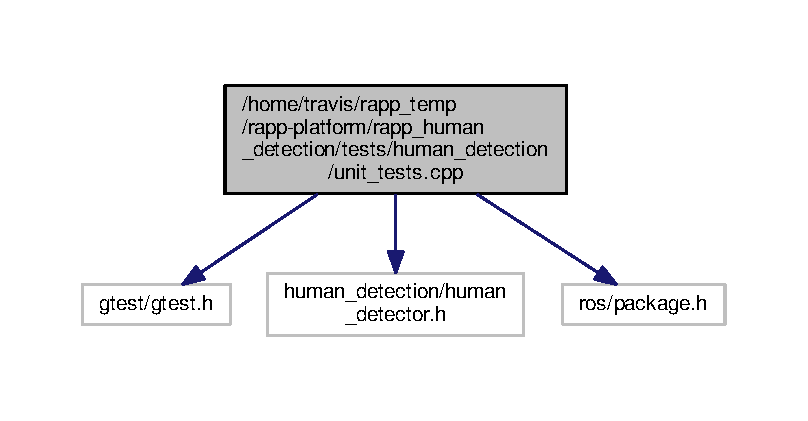
\includegraphics[width=350pt]{unit__tests_8cpp__incl}
\end{center}
\end{figure}
\subsection*{Classes}
\begin{DoxyCompactItemize}
\item 
class \hyperlink{classDoorCheckTest}{Door\-Check\-Test}
\begin{DoxyCompactList}\small\item\em Handles the door angle detection unit testing using gtests. \end{DoxyCompactList}\item 
class \hyperlink{classLightCheckTest}{Light\-Check\-Test}
\begin{DoxyCompactList}\small\item\em Handles the light cheking unit testing using gtests. \end{DoxyCompactList}\end{DoxyCompactItemize}
\subsection*{Functions}
\begin{DoxyCompactItemize}
\item 
int \hyperlink{unit__tests_8cpp_a3c04138a5bfe5d72780bb7e82a18e627}{main} (int argc, char $\ast$$\ast$argv)
\begin{DoxyCompactList}\small\item\em The main function. Initialized the unit tests. \end{DoxyCompactList}\item 
\hyperlink{unit__tests_8cpp_a25497651dab20e8ce0c7f5b6d9c36534}{T\-E\-S\-T\-\_\-\-F} (\hyperlink{classLightCheckTest}{Light\-Check\-Test}, test\-\_\-on)
\begin{DoxyCompactList}\small\item\em Tests light detection with the lamp turned on. Should be successful. \end{DoxyCompactList}\item 
\hyperlink{unit__tests_8cpp_a99b4a483ee6f83a28e90dfb96761122f}{T\-E\-S\-T\-\_\-\-F} (\hyperlink{classLightCheckTest}{Light\-Check\-Test}, test\-\_\-off)
\begin{DoxyCompactList}\small\item\em Tests light detection with the lamp turned off. Should be successful. \end{DoxyCompactList}\item 
\hyperlink{unit__tests_8cpp_a765c0269469869caada3b4bf40d5398c}{T\-E\-S\-T\-\_\-\-F} (\hyperlink{classLightCheckTest}{Light\-Check\-Test}, test\-\_\-size)
\begin{DoxyCompactList}\small\item\em Tests light detection on the same image with different scales. \end{DoxyCompactList}\item 
\hyperlink{unit__tests_8cpp_ac37517df2c7876ecc3e2e9dec76c5490}{T\-E\-S\-T\-\_\-\-F} (\hyperlink{classLightCheckTest}{Light\-Check\-Test}, file\-\_\-not\-\_\-exists\-\_\-test)
\begin{DoxyCompactList}\small\item\em Tests light detection with a missing file. Should return 0. \end{DoxyCompactList}\item 
\hyperlink{unit__tests_8cpp_a92f4df6beb0723cdd1511ec98d578279}{T\-E\-S\-T\-\_\-\-F} (\hyperlink{classDoorCheckTest}{Door\-Check\-Test}, file\-\_\-not\-\_\-exists\-\_\-test)
\begin{DoxyCompactList}\small\item\em Tests door angle detection with a missing file. Should return 0. \end{DoxyCompactList}\item 
\hyperlink{unit__tests_8cpp_a3d24d8e3eb46dbdeb2a8fa0715ce3de8}{T\-E\-S\-T\-\_\-\-F} (\hyperlink{classDoorCheckTest}{Door\-Check\-Test}, door\-\_\-open\-\_\-test)
\begin{DoxyCompactList}\small\item\em Tests door angle detection with a example file. Should return positive value. \end{DoxyCompactList}\end{DoxyCompactItemize}


\subsection{Function Documentation}
\hypertarget{unit__tests_8cpp_a3c04138a5bfe5d72780bb7e82a18e627}{\index{unit\-\_\-tests.\-cpp@{unit\-\_\-tests.\-cpp}!main@{main}}
\index{main@{main}!unit_tests.cpp@{unit\-\_\-tests.\-cpp}}
\subsubsection[{main}]{\setlength{\rightskip}{0pt plus 5cm}int main (
\begin{DoxyParamCaption}
\item[{int}]{argc, }
\item[{char $\ast$$\ast$}]{argv}
\end{DoxyParamCaption}
)}}\label{unit__tests_8cpp_a3c04138a5bfe5d72780bb7e82a18e627}


The main function. Initialized the unit tests. 



Definition at line 167 of file unit\-\_\-tests.\-cpp.

\hypertarget{unit__tests_8cpp_a25497651dab20e8ce0c7f5b6d9c36534}{\index{unit\-\_\-tests.\-cpp@{unit\-\_\-tests.\-cpp}!T\-E\-S\-T\-\_\-\-F@{T\-E\-S\-T\-\_\-\-F}}
\index{T\-E\-S\-T\-\_\-\-F@{T\-E\-S\-T\-\_\-\-F}!unit_tests.cpp@{unit\-\_\-tests.\-cpp}}
\subsubsection[{T\-E\-S\-T\-\_\-\-F}]{\setlength{\rightskip}{0pt plus 5cm}T\-E\-S\-T\-\_\-\-F (
\begin{DoxyParamCaption}
\item[{{\bf Light\-Check\-Test}}]{, }
\item[{test\-\_\-on}]{}
\end{DoxyParamCaption}
)}}\label{unit__tests_8cpp_a25497651dab20e8ce0c7f5b6d9c36534}


Tests light detection with the lamp turned on. Should be successful. 



Definition at line 61 of file unit\-\_\-tests.\-cpp.

\hypertarget{unit__tests_8cpp_a99b4a483ee6f83a28e90dfb96761122f}{\index{unit\-\_\-tests.\-cpp@{unit\-\_\-tests.\-cpp}!T\-E\-S\-T\-\_\-\-F@{T\-E\-S\-T\-\_\-\-F}}
\index{T\-E\-S\-T\-\_\-\-F@{T\-E\-S\-T\-\_\-\-F}!unit_tests.cpp@{unit\-\_\-tests.\-cpp}}
\subsubsection[{T\-E\-S\-T\-\_\-\-F}]{\setlength{\rightskip}{0pt plus 5cm}T\-E\-S\-T\-\_\-\-F (
\begin{DoxyParamCaption}
\item[{{\bf Light\-Check\-Test}}]{, }
\item[{test\-\_\-off}]{}
\end{DoxyParamCaption}
)}}\label{unit__tests_8cpp_a99b4a483ee6f83a28e90dfb96761122f}


Tests light detection with the lamp turned off. Should be successful. 



Definition at line 72 of file unit\-\_\-tests.\-cpp.

\hypertarget{unit__tests_8cpp_a765c0269469869caada3b4bf40d5398c}{\index{unit\-\_\-tests.\-cpp@{unit\-\_\-tests.\-cpp}!T\-E\-S\-T\-\_\-\-F@{T\-E\-S\-T\-\_\-\-F}}
\index{T\-E\-S\-T\-\_\-\-F@{T\-E\-S\-T\-\_\-\-F}!unit_tests.cpp@{unit\-\_\-tests.\-cpp}}
\subsubsection[{T\-E\-S\-T\-\_\-\-F}]{\setlength{\rightskip}{0pt plus 5cm}T\-E\-S\-T\-\_\-\-F (
\begin{DoxyParamCaption}
\item[{{\bf Light\-Check\-Test}}]{, }
\item[{test\-\_\-size}]{}
\end{DoxyParamCaption}
)}}\label{unit__tests_8cpp_a765c0269469869caada3b4bf40d5398c}


Tests light detection on the same image with different scales. 



Definition at line 84 of file unit\-\_\-tests.\-cpp.

\hypertarget{unit__tests_8cpp_ac37517df2c7876ecc3e2e9dec76c5490}{\index{unit\-\_\-tests.\-cpp@{unit\-\_\-tests.\-cpp}!T\-E\-S\-T\-\_\-\-F@{T\-E\-S\-T\-\_\-\-F}}
\index{T\-E\-S\-T\-\_\-\-F@{T\-E\-S\-T\-\_\-\-F}!unit_tests.cpp@{unit\-\_\-tests.\-cpp}}
\subsubsection[{T\-E\-S\-T\-\_\-\-F}]{\setlength{\rightskip}{0pt plus 5cm}T\-E\-S\-T\-\_\-\-F (
\begin{DoxyParamCaption}
\item[{{\bf Light\-Check\-Test}}]{, }
\item[{file\-\_\-not\-\_\-exists\-\_\-test}]{}
\end{DoxyParamCaption}
)}}\label{unit__tests_8cpp_ac37517df2c7876ecc3e2e9dec76c5490}


Tests light detection with a missing file. Should return 0. 



Definition at line 97 of file unit\-\_\-tests.\-cpp.

\hypertarget{unit__tests_8cpp_a92f4df6beb0723cdd1511ec98d578279}{\index{unit\-\_\-tests.\-cpp@{unit\-\_\-tests.\-cpp}!T\-E\-S\-T\-\_\-\-F@{T\-E\-S\-T\-\_\-\-F}}
\index{T\-E\-S\-T\-\_\-\-F@{T\-E\-S\-T\-\_\-\-F}!unit_tests.cpp@{unit\-\_\-tests.\-cpp}}
\subsubsection[{T\-E\-S\-T\-\_\-\-F}]{\setlength{\rightskip}{0pt plus 5cm}T\-E\-S\-T\-\_\-\-F (
\begin{DoxyParamCaption}
\item[{{\bf Door\-Check\-Test}}]{, }
\item[{file\-\_\-not\-\_\-exists\-\_\-test}]{}
\end{DoxyParamCaption}
)}}\label{unit__tests_8cpp_a92f4df6beb0723cdd1511ec98d578279}


Tests door angle detection with a missing file. Should return 0. 



Definition at line 145 of file unit\-\_\-tests.\-cpp.

\hypertarget{unit__tests_8cpp_a3d24d8e3eb46dbdeb2a8fa0715ce3de8}{\index{unit\-\_\-tests.\-cpp@{unit\-\_\-tests.\-cpp}!T\-E\-S\-T\-\_\-\-F@{T\-E\-S\-T\-\_\-\-F}}
\index{T\-E\-S\-T\-\_\-\-F@{T\-E\-S\-T\-\_\-\-F}!unit_tests.cpp@{unit\-\_\-tests.\-cpp}}
\subsubsection[{T\-E\-S\-T\-\_\-\-F}]{\setlength{\rightskip}{0pt plus 5cm}T\-E\-S\-T\-\_\-\-F (
\begin{DoxyParamCaption}
\item[{{\bf Door\-Check\-Test}}]{, }
\item[{door\-\_\-open\-\_\-test}]{}
\end{DoxyParamCaption}
)}}\label{unit__tests_8cpp_a3d24d8e3eb46dbdeb2a8fa0715ce3de8}


Tests door angle detection with a example file. Should return positive value. 



Definition at line 156 of file unit\-\_\-tests.\-cpp.


%--- End generated contents ---

% Index
\newpage
\phantomsection
\addcontentsline{toc}{chapter}{Index}
\printindex

\end{document}
